\subsection{Switch sizing} \label{switch_sizing}

The system must regulate the power flow in order to maximize the power generation. In order to achieve this, the system includes switches that control the current flow. The switches consist on MOSFET devices. The switching frequency of the system is $50 $ kHz. Although the market has IGBT which can switch at $50$ kHz, MOSFET devices allow lower losses than IGBTs for system's current rating. \cite{mosfet_igbt_switching_loss} \cite{igbt_or_mosfet}

The maximum output voltage of the system is $90 $V, however the voltage rating of the transistors was set to $150 $V in order to increase the reliability. The peak current through the transistors happens when the buck mode is activated. The peak current is equal to $14$ A\todo{check with jesper if hhe did this calculation and then link, if not I calculated and have a photo of it}. In order to reduce the conduction losses and the heat sink size, a low on resistance is desired. This constraints were used when searching for the ideal component. The chosen device is the IPB200N15N3. It exhibits the features seen in table \ref{mosfet_features}.

\begin{table}[htbp]
	\centering
	\begin{tabular}{|p{6cm}|>{\centering}p{8cm}|}
		\hline
		\rowcolor{lightgray}\multicolumn{2}{|l|}{ \textbf{Maximum ratings}} \\ \hline
		Continuous $I_{D}$ & 40 [A]  \tabularnewline \hline
		$V_{GS}$ & $\pm$ 20 [V]  \tabularnewline \hline
		Power dissipation & 150 [W]  \tabularnewline \hline
		$V_{DS}$ & 150 [V]  \tabularnewline \hline
		$R_{DSon} $ & 20 [m$\Omega$]  \tabularnewline \hline
		\rowcolor{lightgray}\multicolumn{2}{|l|}{ \textbf{Other values of interest}} \\ \hline
		$C_{GS} $ & 1.81 [nF]  \tabularnewline \hline
		Package & D2PAK  \tabularnewline \hline
	
	\end{tabular}
	\caption{MOSFET figures of merit. T = 25 $\decC$. \cite{mosfet_datasheet}}
	\label{mosfet_features}
\end{table}

\subsection{Heat sink sizing}

The power dissipated in the switches is equal to the sum of the conduction losses and the switching losses. The conduction loss might be calculated  as seen in equation \ref{conduction_losses_eq}.

\begin{equation} \label{conduction_losses_eq}
P_{cond} = i(t)^2 \cdot R_{DS}
\end{equation}


The switching losses depend upon the switching frequency and the transistor's manufacturing characteristics. In order to calculate the value, the MOSFET's SPICE model was obtained from the manufacturer's website. The next step was to perform the simulation of the system. The system was simulated in both Buck and Boost modes. Special attention was put into the dead-band between PWM signals of different switches, to avoid current shoot through. After simulating, the average power dissipation under steady state was calculated in both Buck and Boost modes. Within every mode, the simulation was performed under the most unfavorable conditions, this is: Buck's output is 24 V and Boost's output is 90 V. The results can be seen in table \ref{mosfet_power_consumption}.

$R_{DS}$ is mainly dependant on the temperature. The models found neglect the temperature difference. Then, in order to get an approximated value considering temperature, the procedure will be to calculate the total losses at constant temperature using the SPICE model and then add the additional conduction losses due to the increase of the resistance, as expressed by equation \ref{total_losses}.

\begin{table}[htbp]
	\centering
	\begin{tabular}{|p{6cm}|>{\centering}p{8cm}|}
		\hline
		\rowcolor{lightgray}\multicolumn{2}{|l|}{ \textbf{Buck Mode}} \\ \hline
		M1 & 2.91 [W]  \tabularnewline \hline
		M2 & 0.82 [W]  \tabularnewline \hline
		M3 & 1.81 [W]  \tabularnewline \hline
		M4 & 0 [W]  \tabularnewline \hline
		Total & 5.54 [W]  \tabularnewline \hline
		\rowcolor{lightgray}\multicolumn{2}{|l|}{ \textbf{Boost Mode}} \\ \hline
		M1 & 0.69 [W]  \tabularnewline \hline
		M2 & 0 [W]  \tabularnewline \hline		
		M3 & 0.48 [W]  \tabularnewline \hline
		M4 & 3.31 [W]  \tabularnewline \hline
		Total & 4.48 [W]  \tabularnewline \hline
	\end{tabular}
	\caption{Average power dissipation in every MOSFET.}
	\label{mosfet_power_consumption}
\end{table}


\begin{equation} \label{total_losses}
\overline{P} = \overline{P_{loss, T = K}} + \overline{i(t)^2 \cdot \Updelta R_{DS}}
\end{equation}

Now the junction temperature based on the power dissipation calculated using the SPICE model is calculated. The case temperature is set to 50 $\decC$, which is considered a realistic scenario. The thermal circuit can be seen in figure \ref{thermal_circuit}. The next step is to choose a commercial heat sink. The constraints are thermal resistance, size and price. TDEX6015/TH was found. Its features might be found in table \ref{heatsink_features}. The switch temperature will be analysed in order to validate the heat sink.

\begin{table}[htbp]
	\centering
	\begin{tabular}{|p{6cm}|>{\centering}p{8cm}|}
		\hline
		\rowcolor{lightgray}\multicolumn{2}{|l|}{ \textbf{Features}} \\ \hline
		Size & 60x60x16 [mm]  \tabularnewline \hline
		Thermal resistance & 2 [K/W]  \tabularnewline \hline
		
	\end{tabular}
	\caption{Heat sink figures of merit.}
	\label{heatsink_features}
\end{table}

\begin{equation} \label{switch_temperature}
T_{J} = T_{housing} + \overline{P_{loss, T = K}} + \cdot  R_{thermal}
\end{equation}

\begin{equation} \label{switch_temperature_w_values}
T_{J} = 50 + 5.54 \cdot  2.06 = 61.41 \decC
\end{equation}

The resistance is calculated as explained in equation \ref{delta_resistance}. The resistance difference is relatively small.

\begin{equation} \label{delta_resistance}
\Updelta R_{DS} = R_{DS, T = 20 \decC} - R_{DS, T = 61.41\decC} = 4\; m \Omega
\end{equation}


\begin{figure}[htbp]
	\begin{center}
		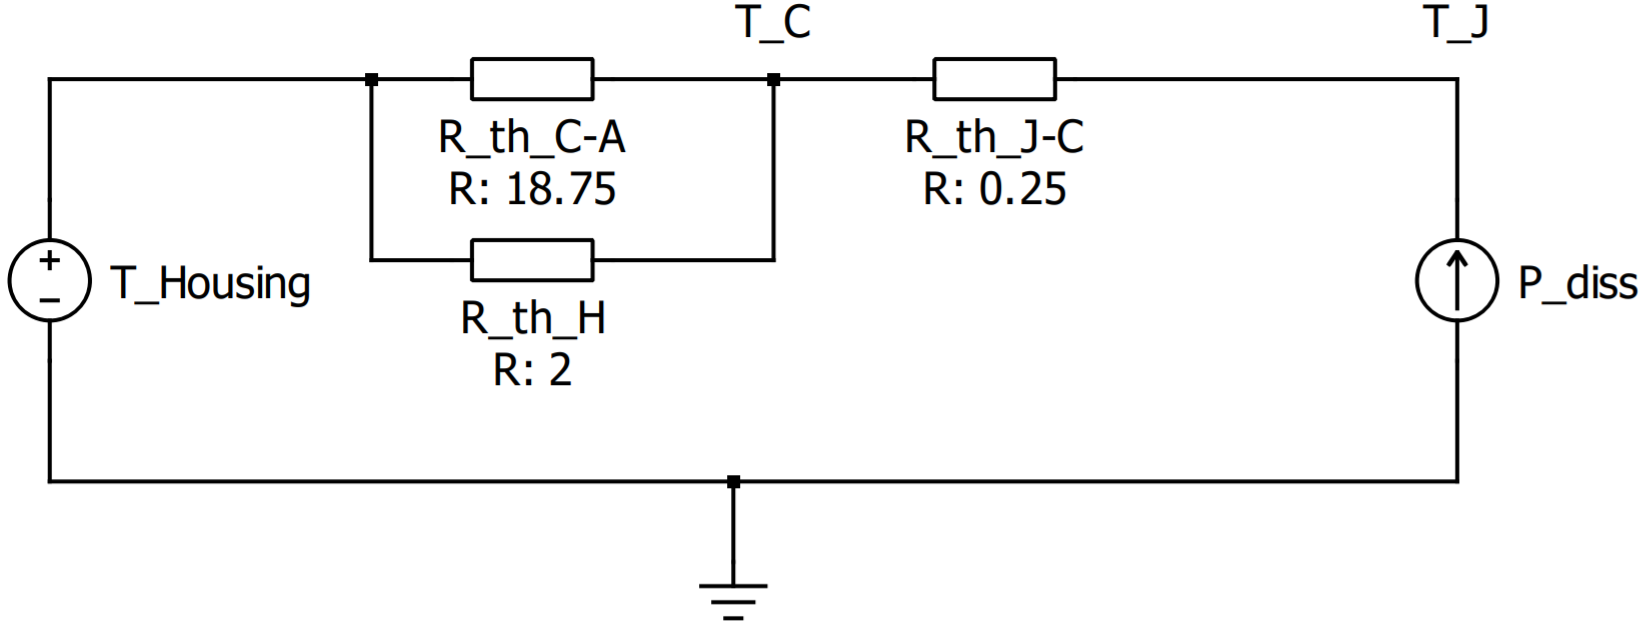
\includegraphics[width=0.4\textwidth]{../Pictures/thermal_circuit.png}
		\caption{Thermal circuit used for sizing the heat sink}
		\label{thermal_circuit}
	\end{center}	
\end{figure}



\begin{table}[]
	\centering
	\begin{tabular}{|l|l|l|l|}
		\hline
		\rowcolor[HTML]{C0C0C0} 
		\multicolumn{4}{|c|}{\cellcolor[HTML]{C0C0C0}\textbf{Switches power dissipation}}                                                   \\ \hline
		\rowcolor[HTML]{C0C0C0} 
		Switch         & $\overline{P_{loss, T = K}}$ {[}W{]} & $ \overline{i(t)^2 \cdot \Updelta R_{DS}}$ {[}W{]} & \textbf{Total {[}W{]}} \\ \hline
		\multicolumn{4}{|l|}{Buck mode}                                                                                                     \\ \hline
		M1             & 2.91                                 & 0.39                                               & \textbf{3.30}          \\ \hline
		M2             & 0.82                                 & 0.21                                               & \textbf{1.03}          \\ \hline
		M3             & 1.81                                 & 0.58                                               & \textbf{2.39}          \\ \hline
		M4             & 0                                    & 0                                                  & \textbf{0}             \\ \hline
		\textbf{Total} & 5.54                                 & 1.18                                               & \textbf{6.72}          \\ \hline
		\multicolumn{4}{|l|}{Boost mode}                                                                                                    \\ \hline
		M1             & 0.69                                 & 0.28                                               & \textbf{0.97}          \\ \hline
		M2             & 0                                    & 0                                                  & \textbf{0}             \\ \hline
		M3             & 0.48                                 & 0.12                                               & \textbf{0.6}           \\ \hline
		M4             & 3.31                                 & 0.18                                               & \textbf{3.49}          \\ \hline
		\textbf{Total} & 4.48                                 & 0.58                                               & \textbf{5.06}          \\ \hline
	\end{tabular}
\caption{Table dissipation including the extra dissipation due to the increase of temperature.}
\label{mosfet_final_dissipation}
\end{table}


The full power dissipation values can be found on table \ref{mosfet_final_dissipation}. To achieve an exact result, the new total power should be used with the thermal circuit in order to calculate again $\Updelta R_{DS}$, but this difference is small and thus neglected. Now that the power dissipation has been calculated, the junction temperature must be checked in order to confirm that the heat sink has been properly sized. Equation \ref{switch_temperature_w_values_2} is used. The difference is fairly small and the junction temperature remains within safe area. Then TDEX6015/TH has been validated as a proper heat sink.

\begin{equation} \label{switch_temperature_w_values_2}
T_{J} = 50 + 6.72 \cdot  2.06 = 63.84 \decC
\end{equation}



